\documentclass[10pt,a4paper]{article}
\usepackage[latin1]{inputenc}
\usepackage{amsmath}
\usepackage{amsfonts}
\usepackage{amssymb}
\usepackage{graphicx}


\usepackage{geometry}
\geometry{left=2.5cm, right=1cm}

\pagenumbering{gobble}

\begin{document}
	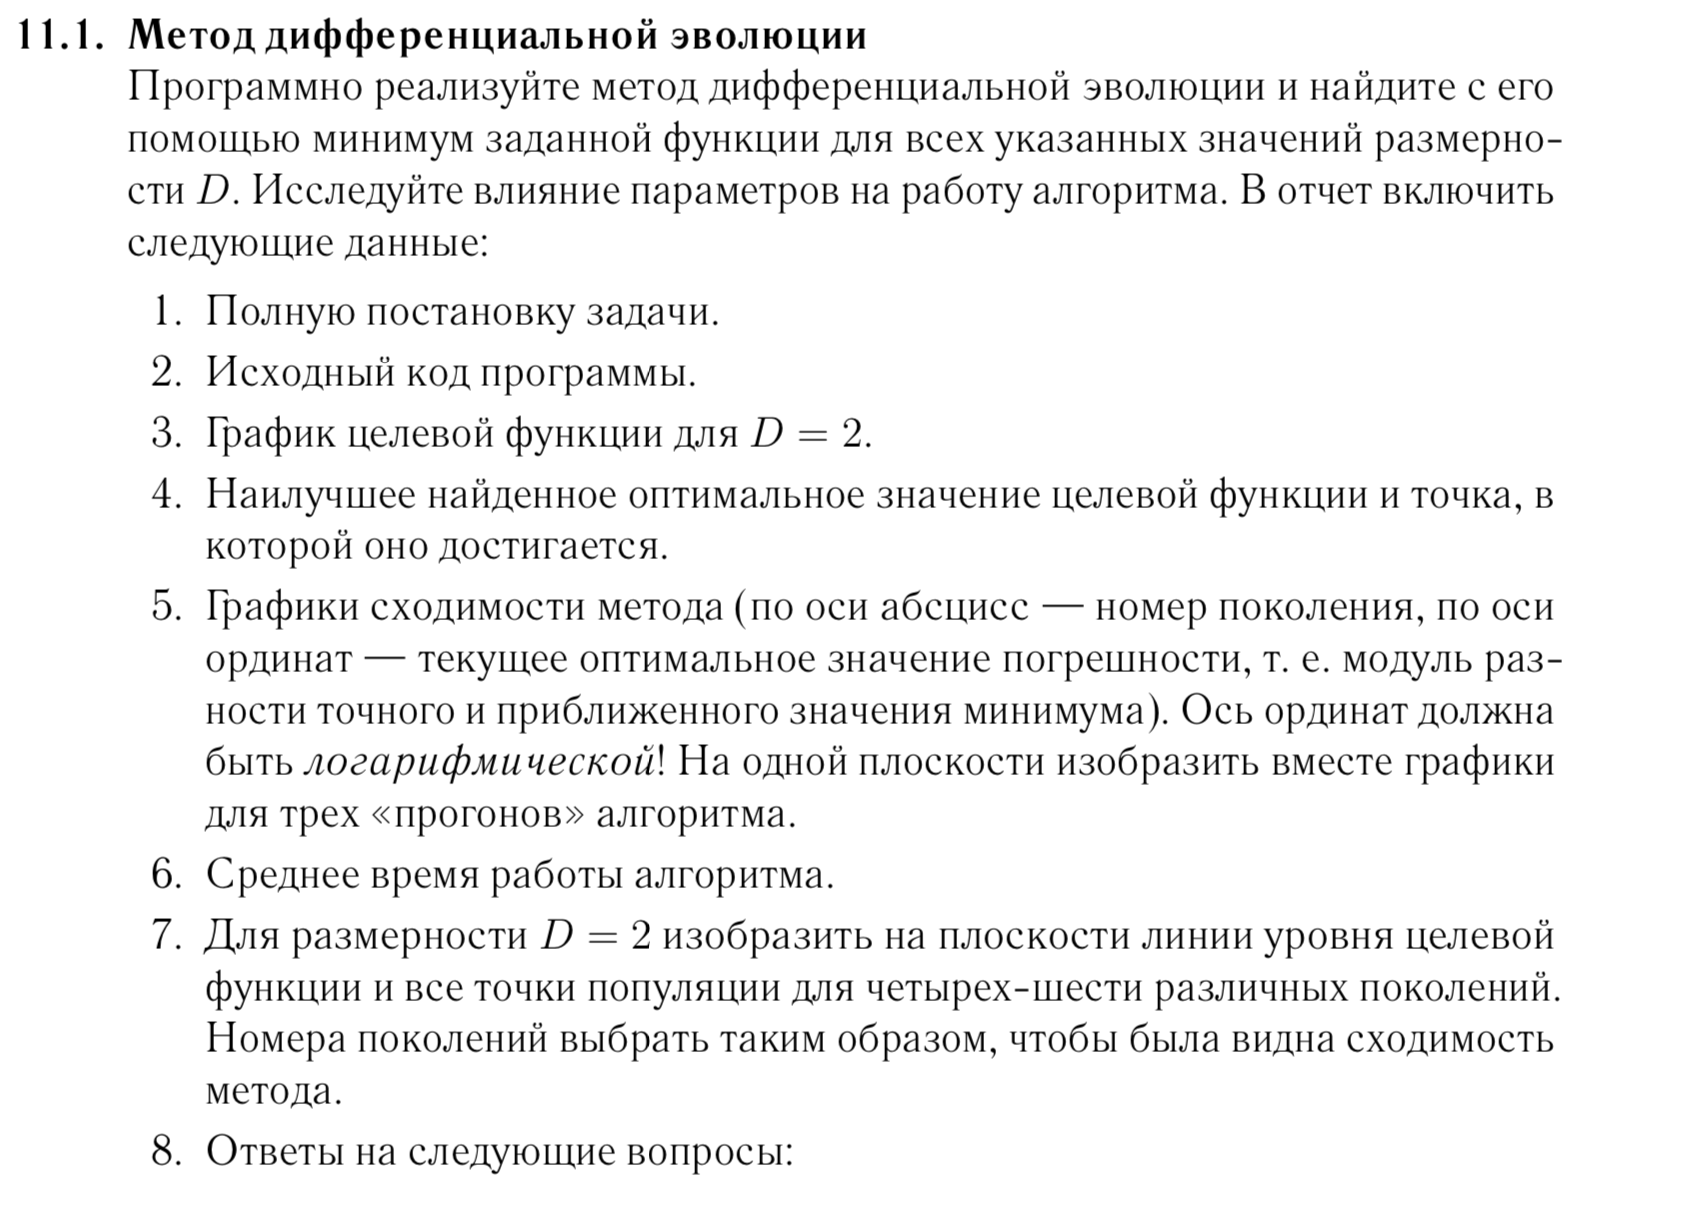
\includegraphics[width=0.8 \textwidth, keepaspectratio]{img/1}
	
	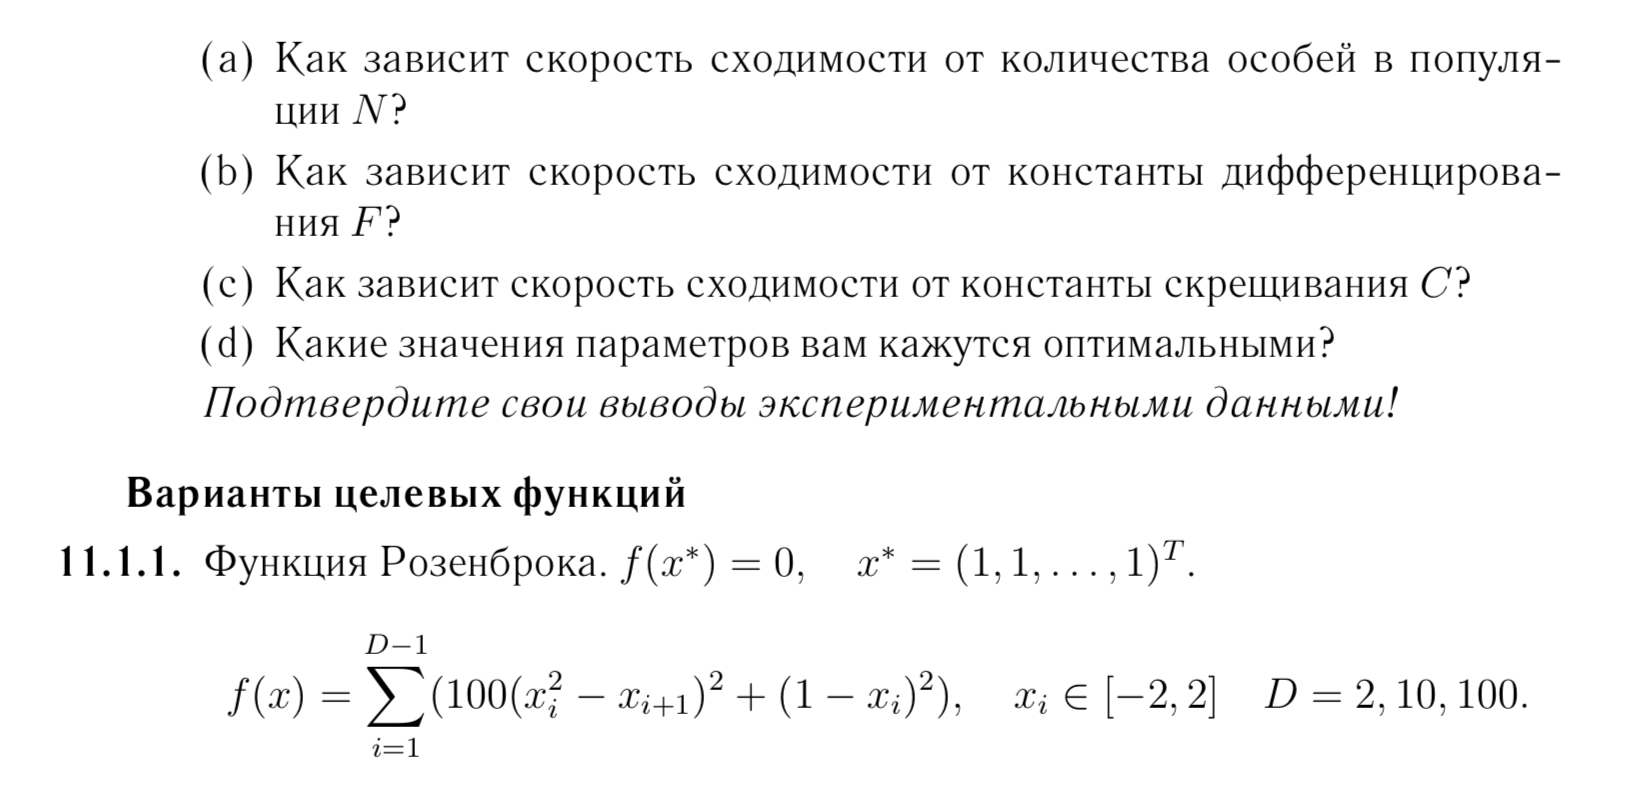
\includegraphics[width=0.8 \textwidth, keepaspectratio]{img/2}
	
	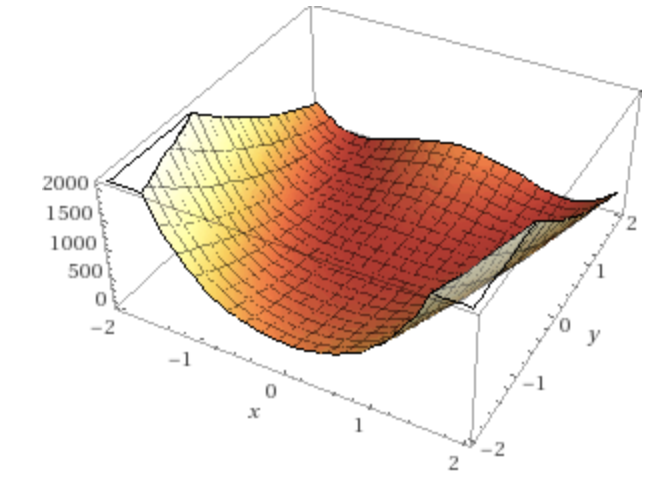
\includegraphics[width= 1 \textwidth, keepaspectratio]{img/3}
	
	\includegraphics[width=  \textwidth, keepaspectratio]{img/4}
	
	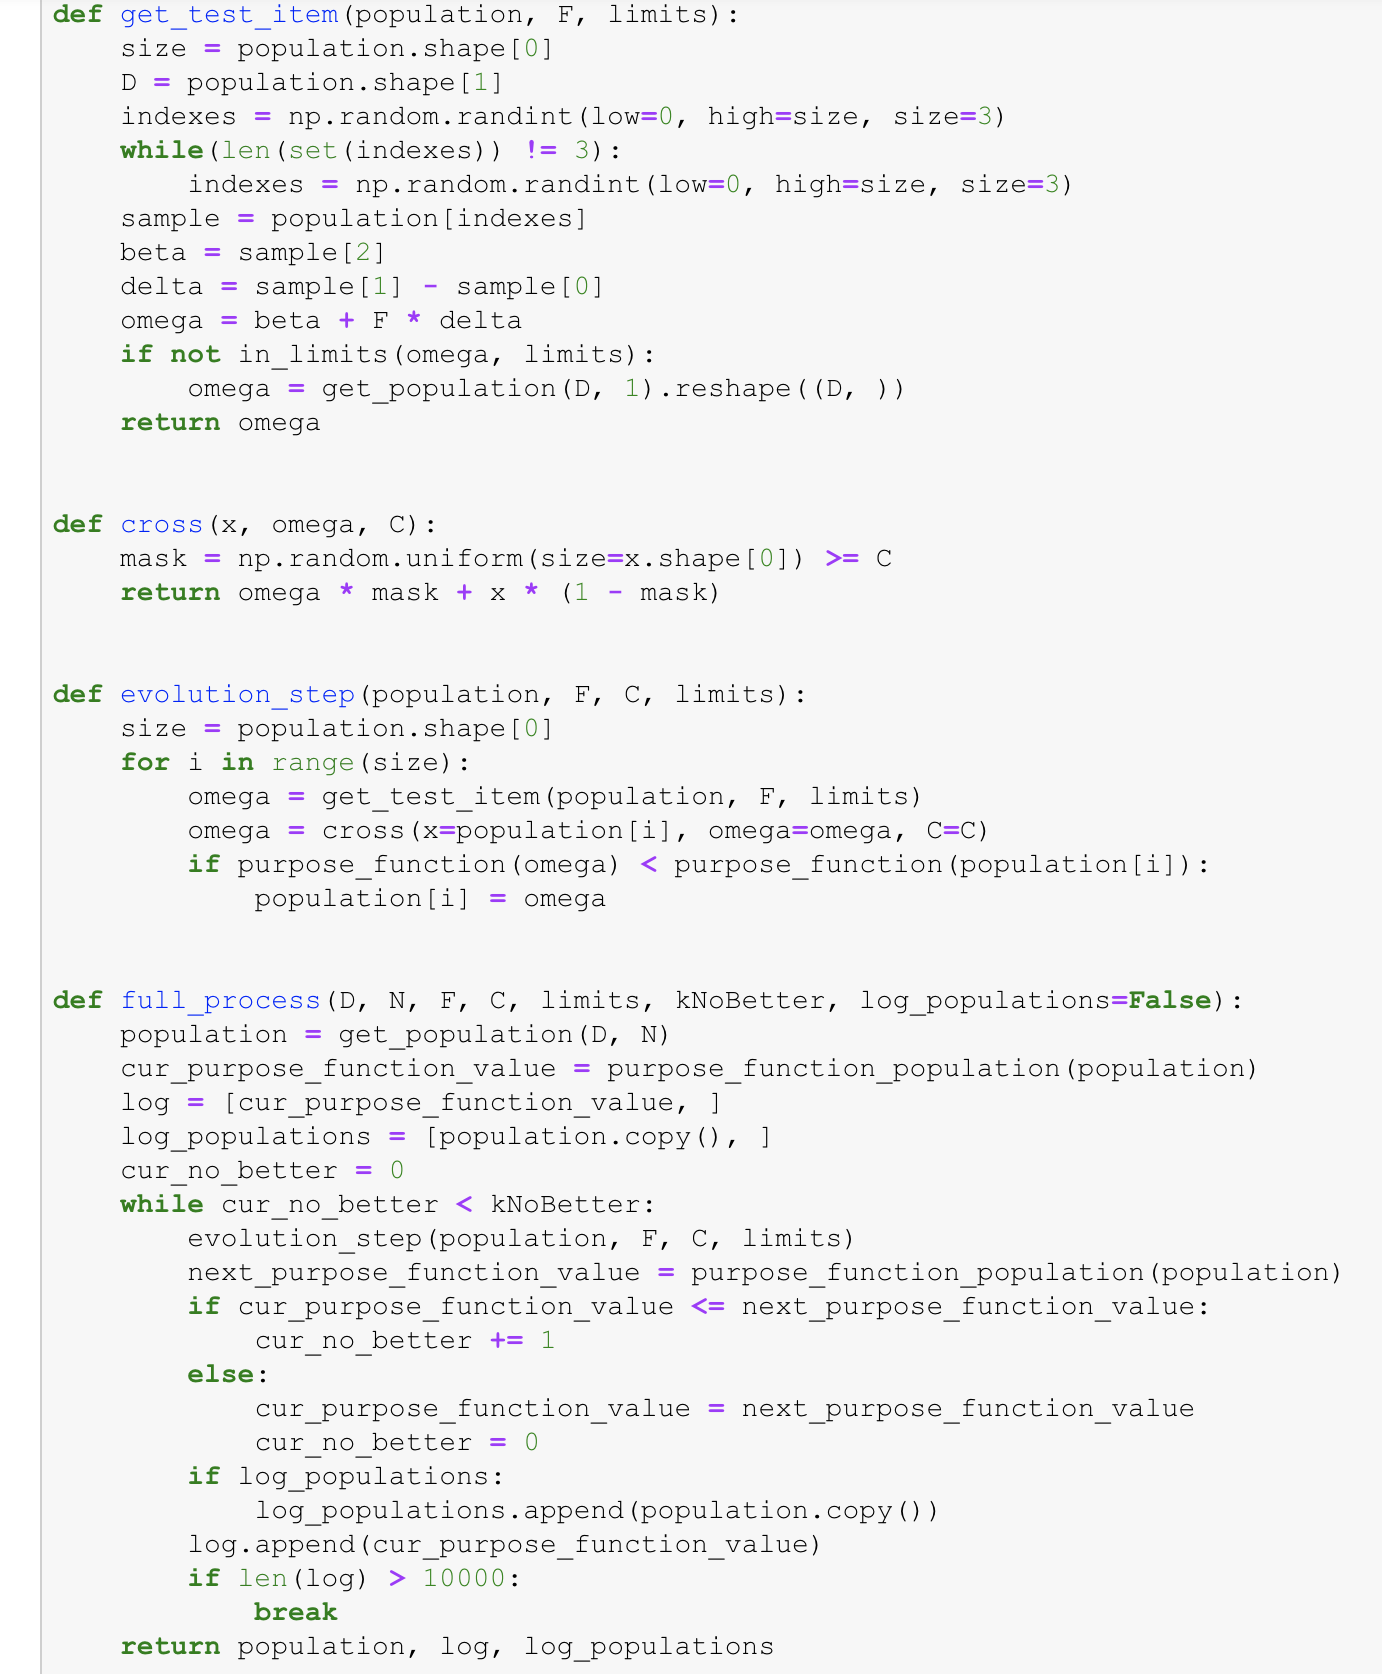
\includegraphics[width= \textwidth, keepaspectratio]{img/5}
	
	
\includegraphics[width= \textwidth, keepaspectratio]{img/6}
	
	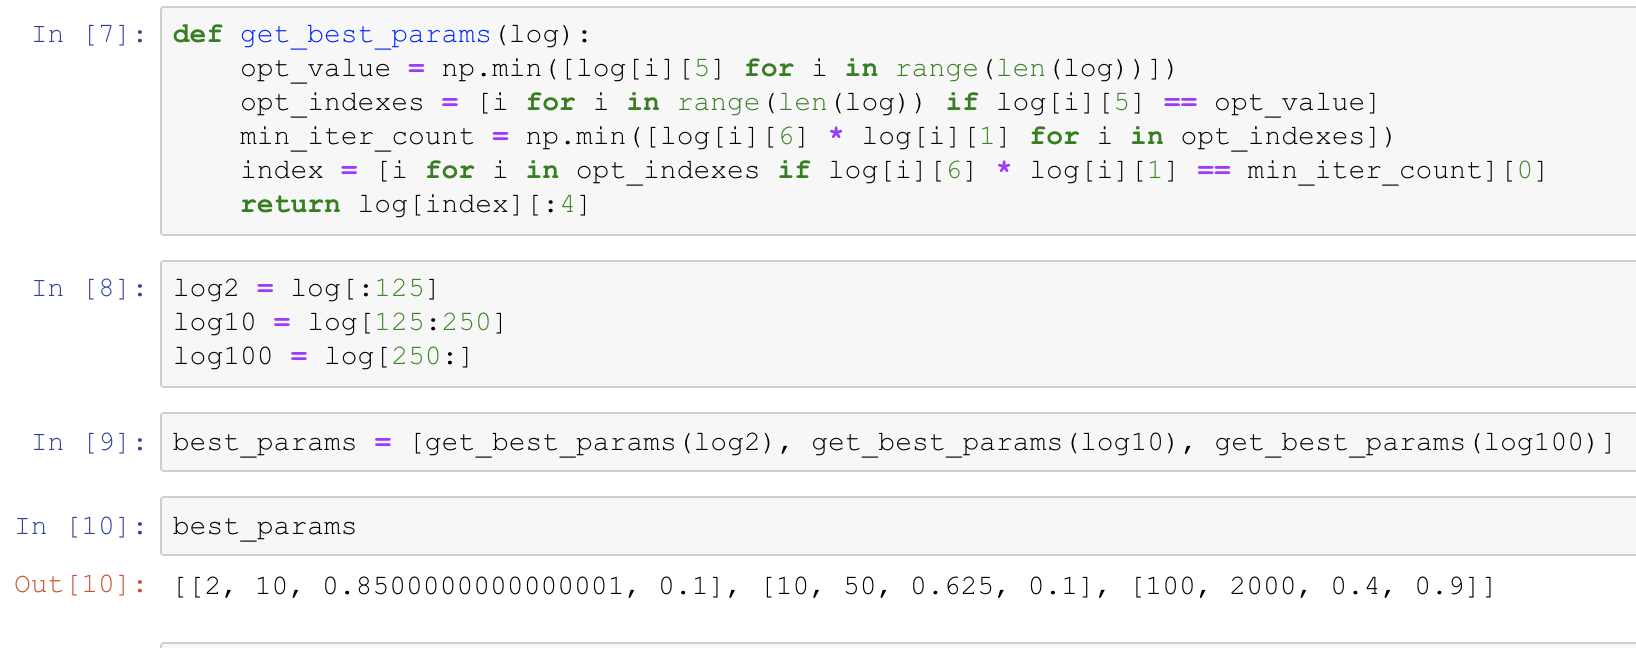
\includegraphics[width= \textwidth, keepaspectratio]{img/7}
	
	\includegraphics[width= \textwidth, keepaspectratio]{img/8}
	
	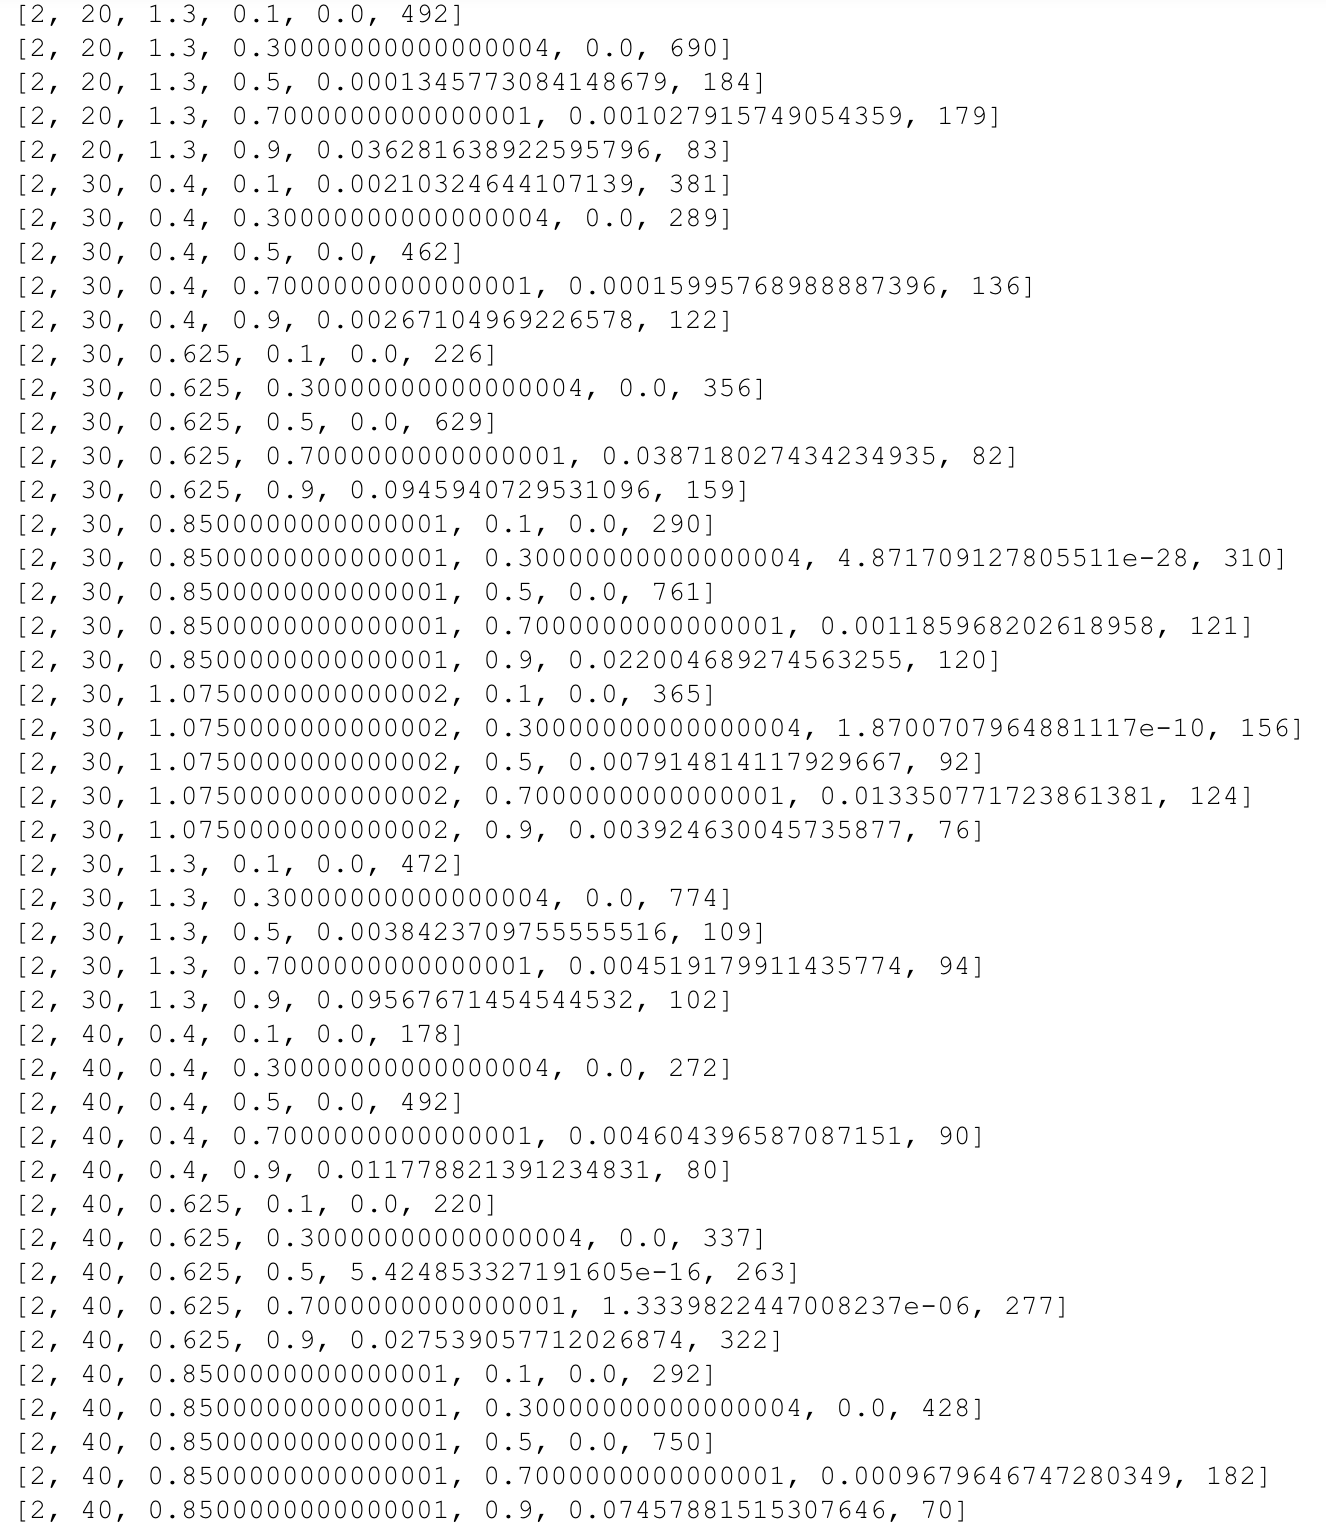
\includegraphics[width= \textwidth, keepaspectratio]{img/9}
	
	\includegraphics[width= \textwidth, keepaspectratio]{img/10}
	
	\includegraphics[width= \textwidth, keepaspectratio]{img/11}
	
	\includegraphics[width= \textwidth, keepaspectratio]{img/12}
	
	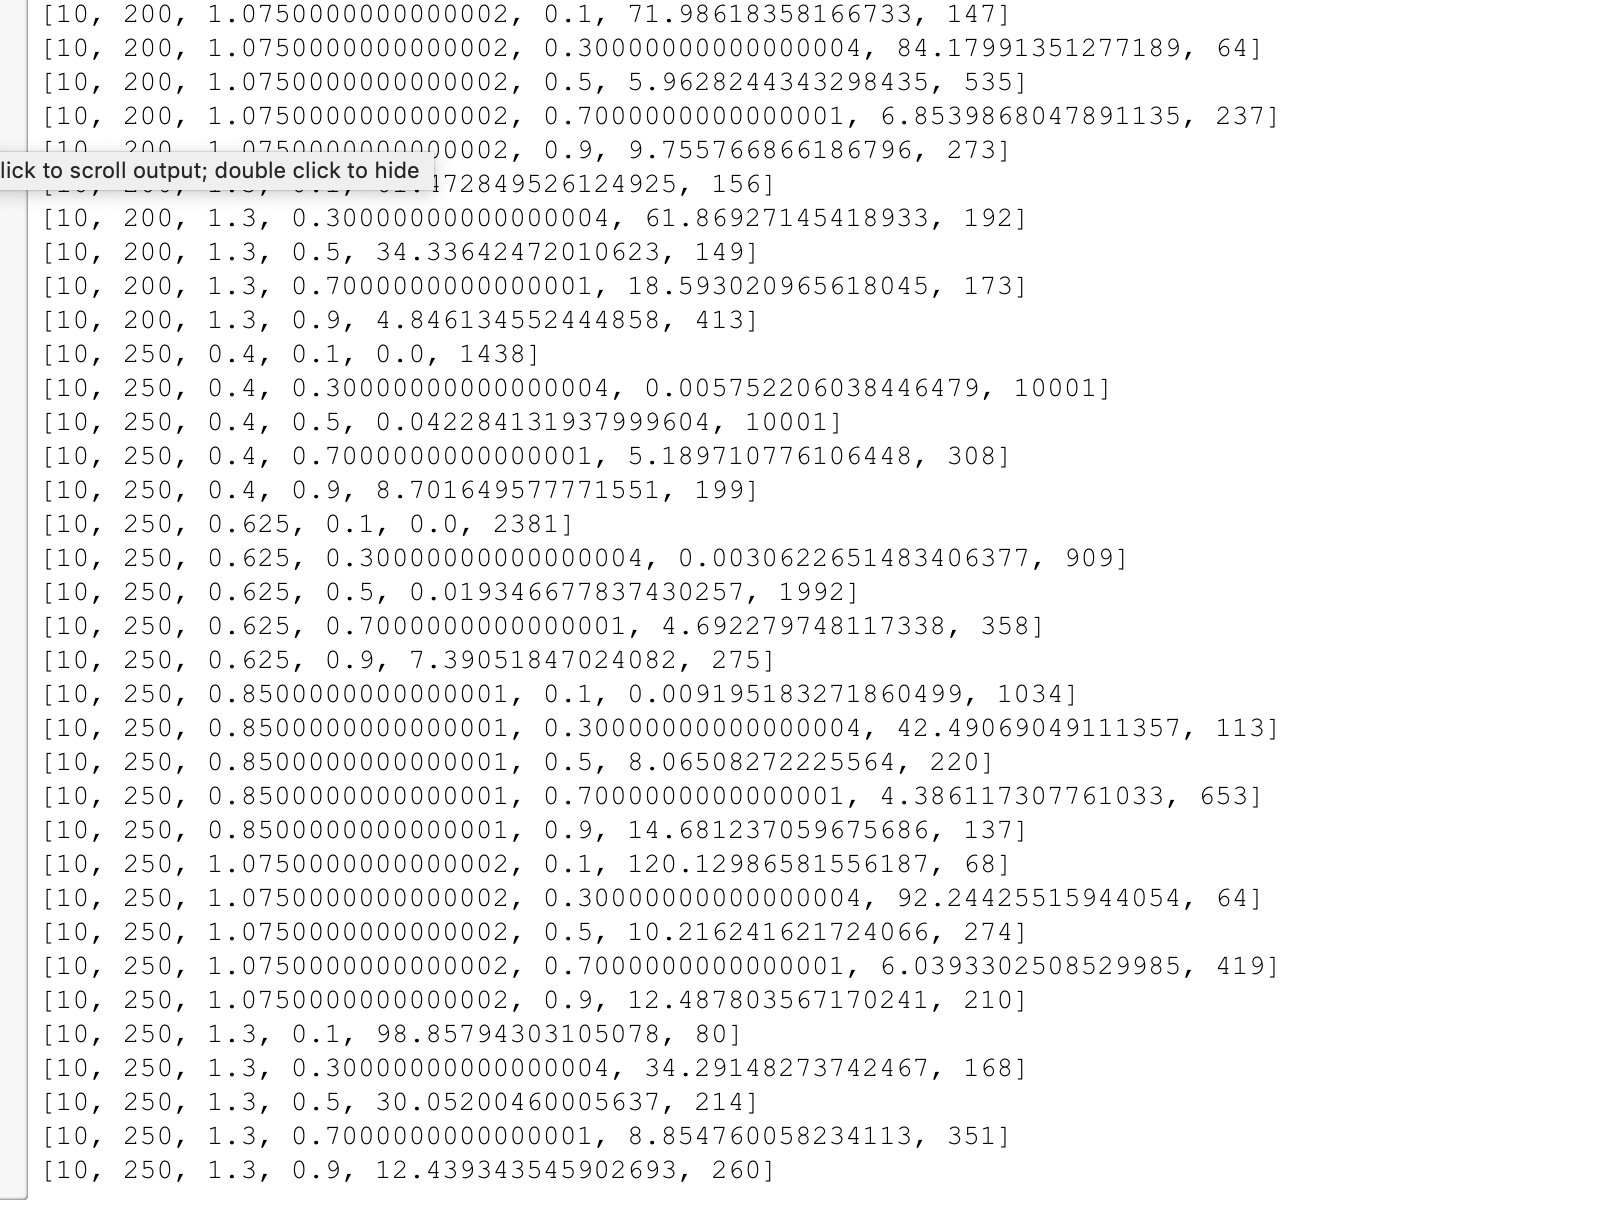
\includegraphics[width= \textwidth, keepaspectratio]{img/13}
	
	\includegraphics[width= \textwidth, keepaspectratio]{img/14}
	
	\includegraphics[width= \textwidth, keepaspectratio]{img/15}
	
	\includegraphics[width= 0.9 \textwidth, keepaspectratio]{img/16}
	
	\includegraphics[width= 0.9 \textwidth, keepaspectratio]{img/17}
	
	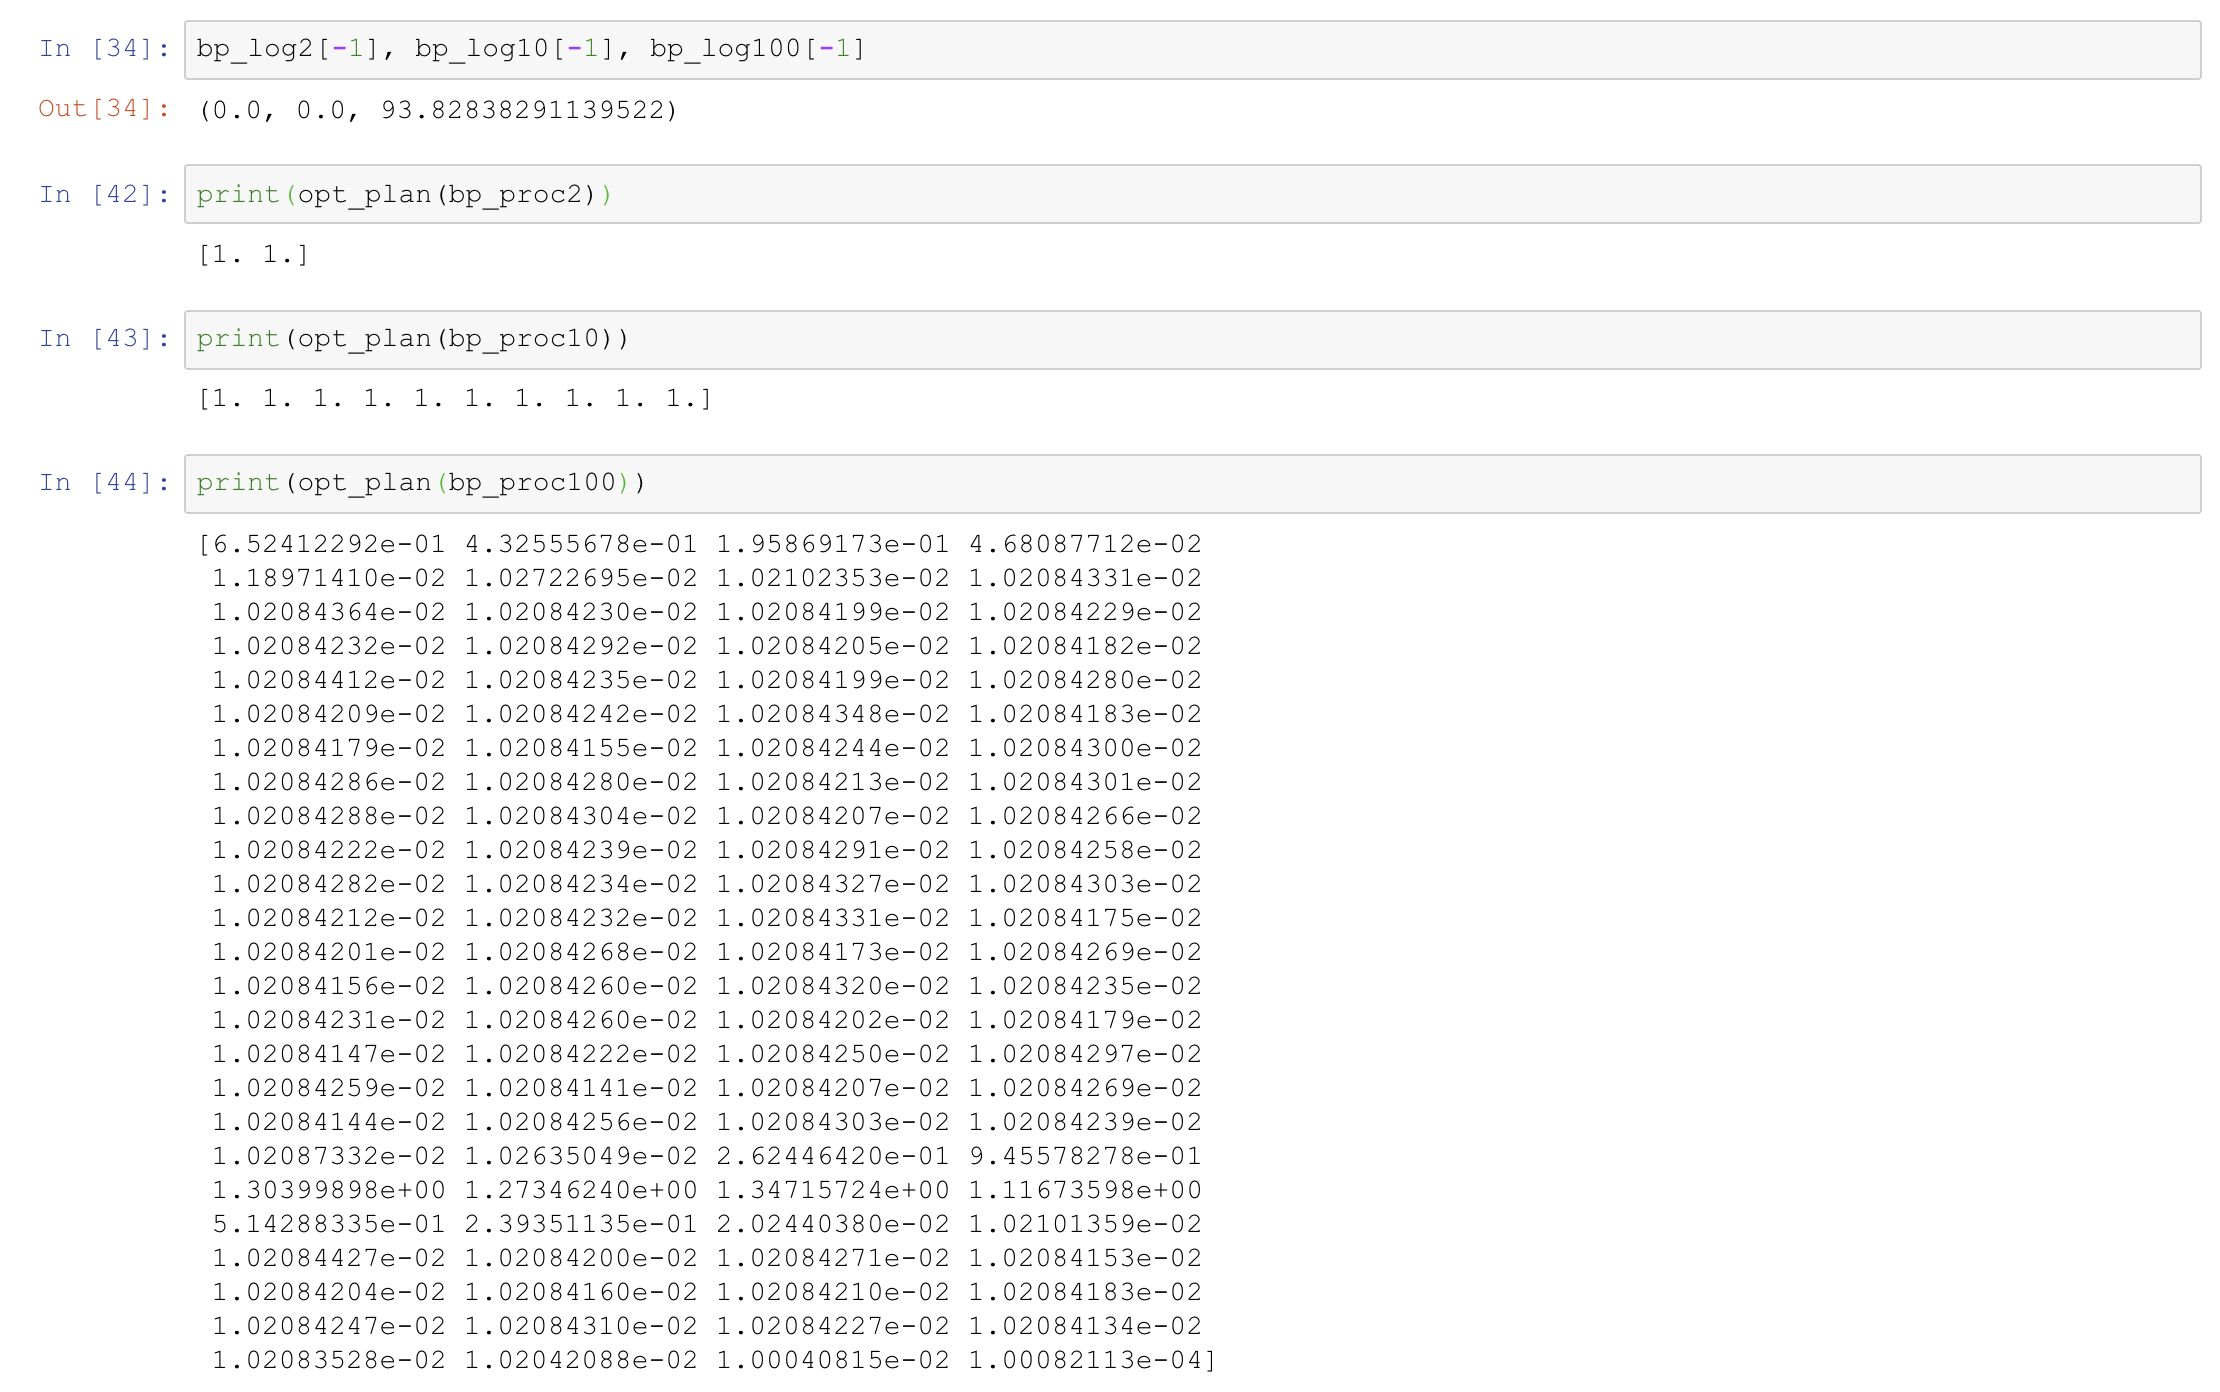
\includegraphics[width= 0.9 \textwidth, keepaspectratio]{img/18}
	
	\includegraphics[width=  \textwidth, keepaspectratio]{img/19}
	
	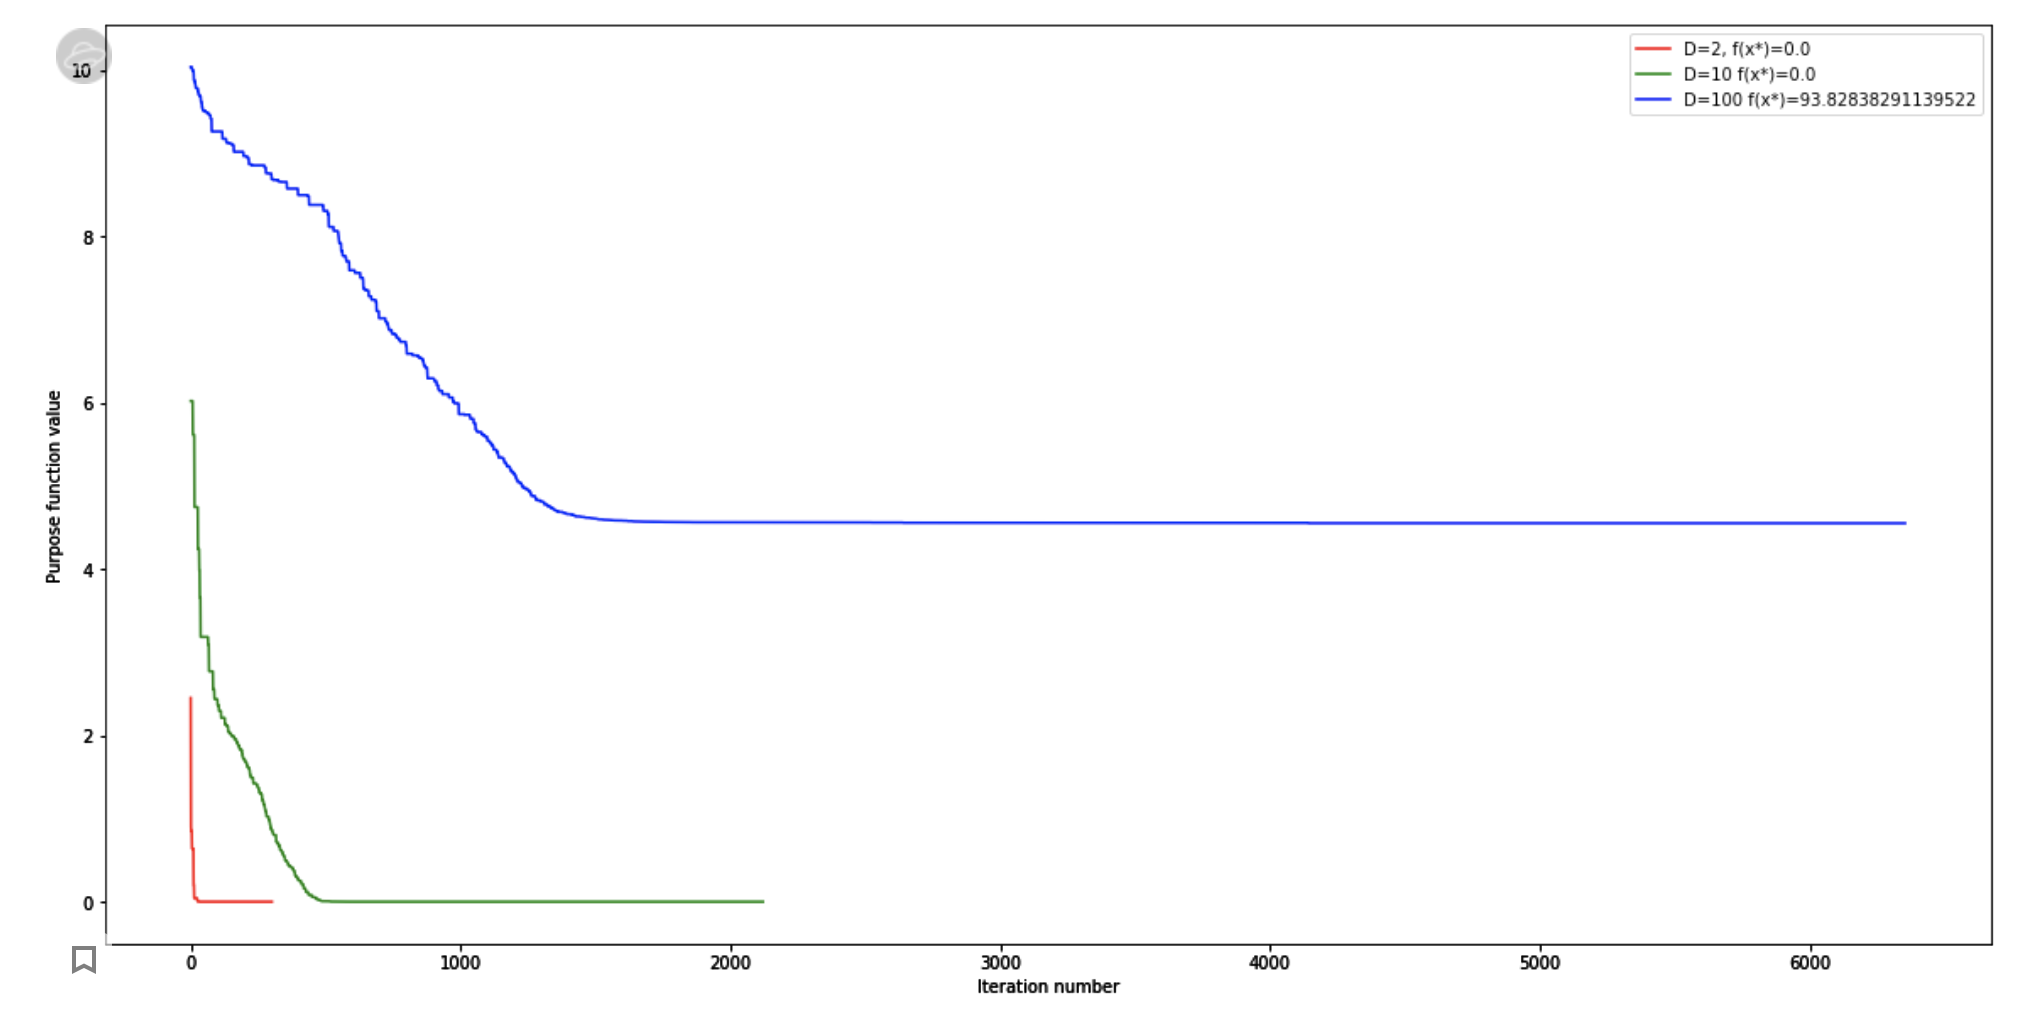
\includegraphics[width=  \textwidth, keepaspectratio]{img/20}
	
	\includegraphics[width=  \textwidth, keepaspectratio]{img/7a}
	
	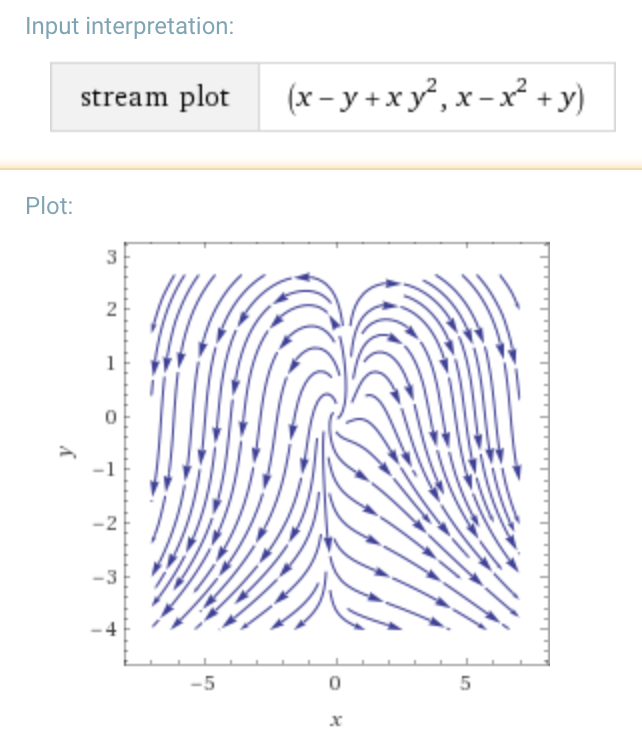
\includegraphics[width=  \textwidth, keepaspectratio]{img/7b}
	
	\includegraphics[width=  \textwidth, keepaspectratio]{img/7c}
\end{document}